\hypertarget{ormulticontrol.cpp-example}{
\subsection{ormulticontrol.cpp}
}
\begin{DoxyAuthor}{Author}
Rosen Diankov
\end{DoxyAuthor}
 
\begin{DoxyImage}
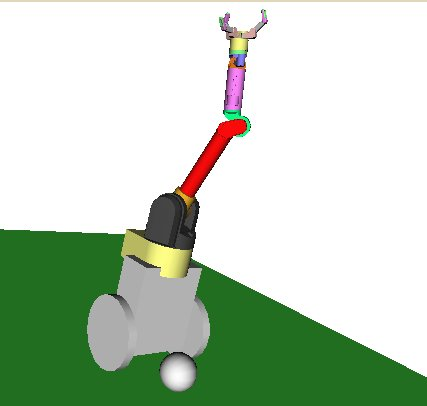
\includegraphics[width=10cm]{cppexample_ormulticontrol.jpg}
\caption{Base moves with velocity control, arm moves with position control.}
\end{DoxyImage}


Shows how to set two controllers for a robot using the MultiController class. The differential base moves with velocity control while the arm moves with position control.

{\bfseries Full Example Code:}


\begin{DoxyCodeInclude}

#include <openrave-core.h>
#include <openrave/planningutils.h>
#include <vector>
#include <cstring>
#include <sstream>

#include <boost/thread/thread.hpp>
#include <boost/bind.hpp>

using namespace OpenRAVE;
using namespace std;

#ifdef _WIN32
#define WIN32_LEAN_AND_MEAN
#include <windows.h>
#define usleep(micro) Sleep(micro/1000)
#endif

void SetViewer(EnvironmentBasePtr penv, const string& viewername)
{
    ViewerBasePtr viewer = RaveCreateViewer(penv,viewername);
    penv->AddViewer(viewer);
    viewer->main(true);
}

int main(int argc, char ** argv)
{
    string scenefilename = "data/diffdrive_arm.env.xml";
    string viewername = "qtcoin";
    RaveInitialize(true);
    EnvironmentBasePtr penv = RaveCreateEnvironment();
    penv->SetDebugLevel(Level_Debug);

    boost::thread thviewer(boost::bind(SetViewer,penv,viewername)); // create the
       viewer
    usleep(400000); // wait for the viewer to init

    penv->Load(scenefilename);

    // attach a physics engine
    penv->SetPhysicsEngine(RaveCreatePhysicsEngine(penv,"ode"));
    penv->GetPhysicsEngine()->SetGravity(Vector(0,0,-9.8));

    vector<RobotBasePtr> vrobots;
    penv->GetRobots(vrobots);
    RobotBasePtr probot = vrobots.at(0);
    std::vector<dReal> q;

    vector<int> wheelindices, restindices;
    ControllerBasePtr wheelcontroller, armcontroller;
    // create the controllers, make sure to lock environment!
    {
        EnvironmentMutex::scoped_lock lock(penv->GetMutex()); // lock environment
      

        MultiControllerPtr multi(new MultiController(penv));
        vector<int> dofindices(probot->GetDOF());
        for(int i = 0; i < probot->GetDOF(); ++i) {
            dofindices[i] = i;
        }
        probot->SetController(multi,dofindices,1); // control everything
        // set the velocity controller on all joints that have 'wheel' in their d
      escription
        for(std::vector<KinBody::JointPtr>::const_iterator itjoint = probot->GetJ
      oints().begin(); itjoint != probot->GetJoints().end(); ++itjoint) {
            if( (*itjoint)->GetName().find("wheel") != string::npos ) {
                for(int i = 0; i < (*itjoint)->GetDOF(); ++i) {
                    wheelindices.push_back((*itjoint)->GetDOFIndex()+i);
                }
            }
            else {
                for(int i = 0; i < (*itjoint)->GetDOF(); ++i) {
                    restindices.push_back((*itjoint)->GetDOFIndex()+i);
                }
            }
        }

        if(wheelindices.size() > 0 ) {
            wheelcontroller = RaveCreateController(penv,"odevelocity");
            multi->AttachController(wheelcontroller,wheelindices,0);
        }

        if( restindices.size() > 0 ) {
            armcontroller = RaveCreateController(penv,"idealcontroller");
            multi->AttachController(armcontroller,restindices,0);
        }
        else {
            RAVELOG_WARN("robot needs to have wheels and arm for demo to work\n")
      ;
        }
    }

    while(1) {
        {
            EnvironmentMutex::scoped_lock lock(penv->GetMutex()); // lock environ
      ment

            if( !!armcontroller ) {
                // set a trajectory on the arm and velocity on the wheels
                TrajectoryBasePtr traj = RaveCreateTrajectory(penv,"");
                probot->SetActiveDOFs(restindices);
                ConfigurationSpecification spec = probot->GetActiveConfigurationS
      pecification();
                int timeoffset = spec.AddDeltaTime();
                traj->Init(spec);
                probot->GetActiveDOFValues(q); // get current values
                vector<dReal> vdata(spec.GetDOF(),0);
                std::copy(q.begin(),q.end(),vdata.begin());
                traj->Insert(0,vdata);
                for(int i = 0; i < 4; ++i) {
                    q.at(RaveRandomInt()%restindices.size()) += RaveRandomFloat()
      -0.5; // move a random axis
                }

                // check for collisions
                {
                    RobotBase::RobotStateSaver saver(probot); // add a state save
      r so robot is not moved permenantly
                    probot->SetActiveDOFValues(q);
                    if( probot->CheckSelfCollision() ) { // don't check env colli
      sions since we have physics enabled
                        continue; // robot in collision at final point, so reject
      
                    }
                }

                std::copy(q.begin(),q.end(),vdata.begin());
                vdata.at(timeoffset) = 2; // trajectory takes 2s
                traj->Insert(1,vdata);
                planningutils::RetimeActiveDOFTrajectory(traj,probot,true);
                armcontroller->SetPath(traj);
            }

            if( !!wheelcontroller ) {
                stringstream sout,ss; ss << "setvelocity ";
                for(size_t i = 0; i < wheelindices.size(); ++i) {
                    ss << 2*(RaveRandomFloat()-0.5) << " ";
                }
                if( !wheelcontroller->SendCommand(sout,ss) ) {
                    RAVELOG_WARN("failed to send velocity command\n");
                }
            }
        }

        // unlock the environment and wait for the arm controller to finish (whee
      l controller will never finish)
        if( !armcontroller ) {
            usleep(2000000);
        }
        else {
            while(!armcontroller->IsDone()) {
                usleep(1000);
            }
        }
    }

    thviewer.join(); // wait for the viewer thread to exit
    penv->Destroy(); // destroy
    return 0;
}
\end{DoxyCodeInclude}
 